\subsection{Subsystem $<$Util$>$}
\\
\subsubsection{Detailed Design Diagram}
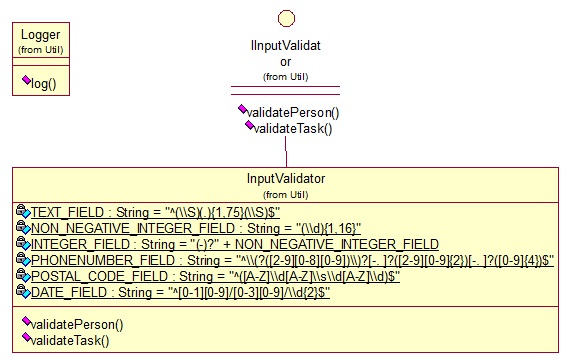
\includegraphics{diagrams/utils_class_diagram}
\\
This package stores all the utility classes needed in the application. Utility classes are classes that are required in multiple components of the application. It contains the Logger, IInputValidator and InputValidator classes.
\\
\subsubsection{Units Description}
\\
\emph{Logger}\\
Functions:\\
\begin{tabular}{| l | l | l | l |}
\hline
Name & Parameters & Pre-conditions & Post-conditions\\
\hline
\multirow{2}{*}{log} & String className, String log & Requires Nothing & Logs \emph{className} and \emph{log} parameters to console
\\&  & & and passed to the main view
\\
\hline
\end{tabular}
\\
Attributes: \emph{none}
\\
Purpose: Its purpose is to log to console the message provided to it. The advantage of a Logger versus directly outputting to console via \emph{System.out.println()} is that it can easily be extended to log to a file without having to made code chage to anywhere else in the application.
\\
\\
\emph{IInputValidator}\\
Functions:\\
\begin{tabular}{| l | l | l | l |}
\hline
Name & Parameters & Pre-conditions & Post-conditions\\
\hline
\multirow{2}{*}{log} & String className, String log & Requires Nothing & Logs \emph{className} and \emph{log} parameters to console\\ 
			 &  & & and passed to the main view
\\
\hline
\end{tabular}
\\
Attributes: \emph{none}
\\
Purpose: Its purpose is to log to console the message provided to it. The advantage of a Logger versus directly outputting to console via \emph{System.out.println()} is that it can easily be extended to log to a file without having to made code chage to anywhere else in the application.
\\
\\
\emph{IInputValidator}\\
Functions:\\
\begin{tabular}{| l | l | l | l |}
\hline
Name & Parameters & Pre-conditions & Post-conditions\\
\hline
\multirow{2}{*}{view} & String path                                 & Requires that path point & Ensures that the tasks have been\\ 
			 & ArrayList$<$Person$>$ people & to a valid location.          & written to the file pointed to by path.\\ 
                                     & ArrayList$<$Task$>$ tasks       &                             & 
\\
\hline
\end{tabular}\\
Purpose: Describe the interface for dumping tasks to a file.